\chapter{Results}
\label{chap4}

All test, for CPU and GPU, had been runned on the same device, the one provided from the course and so all 
results obtain are related to this hardware.

\section{Execution}

To start execution is possible run one of the bash script avaible.

\begin{itemize}
    \item \emph{run.sh}, to tun all the GPU version.
    %\item \emph{run_CPU.sh}, to run all the CPU versions.
    %\item \emph{run_long.sh}, to run a long execution of a particular DFG using the version 4.1, the only that can carry such a load.
\end{itemize}

To run a single version directly three element are needed.

\begin{itemize}
    \item A file containining the DFG infomormation, this file ara obtain through original DFG file savef in .dot format. The converion is achieved throught a pyhton script explained in appendix \ref{appendix1}.
    \item The value of area constrained.
    \item A file containining the all the possible resources avaiable that is organized in the following way:
    \begin{itemize}
        \item first row is the number of operations k;
        \item then there are k rows containining the pair operation number and number n different kind of resources;
        \item after each of this row there are n row containining the pair area and speed of each resources that can execute that operation.
    \end{itemize}
\end{itemize}

The executable can ba run in the following way:

\begin{lstlisting}
\center
    dfg.o <dfg_name>.txt <RTL_file>.txt <area_constrained>
\end{lstlisting}

All latency are avaiable al label according DFG inside a log file.

\section{Comparison}

In the following graphes is possible to observe the performace of the all versions. A lot of other
testbenches had been runned to check not only performances but also the correctness of the scheduling but the ones
show here are the most significant.
It's importantto notice that version 1 is useless because when it works there are not big differences of time
compare to the CPU execution.

\begin{figure}[!h]
    \centering
    \begin{subfigure}{.45\textwidth}
        \centering
        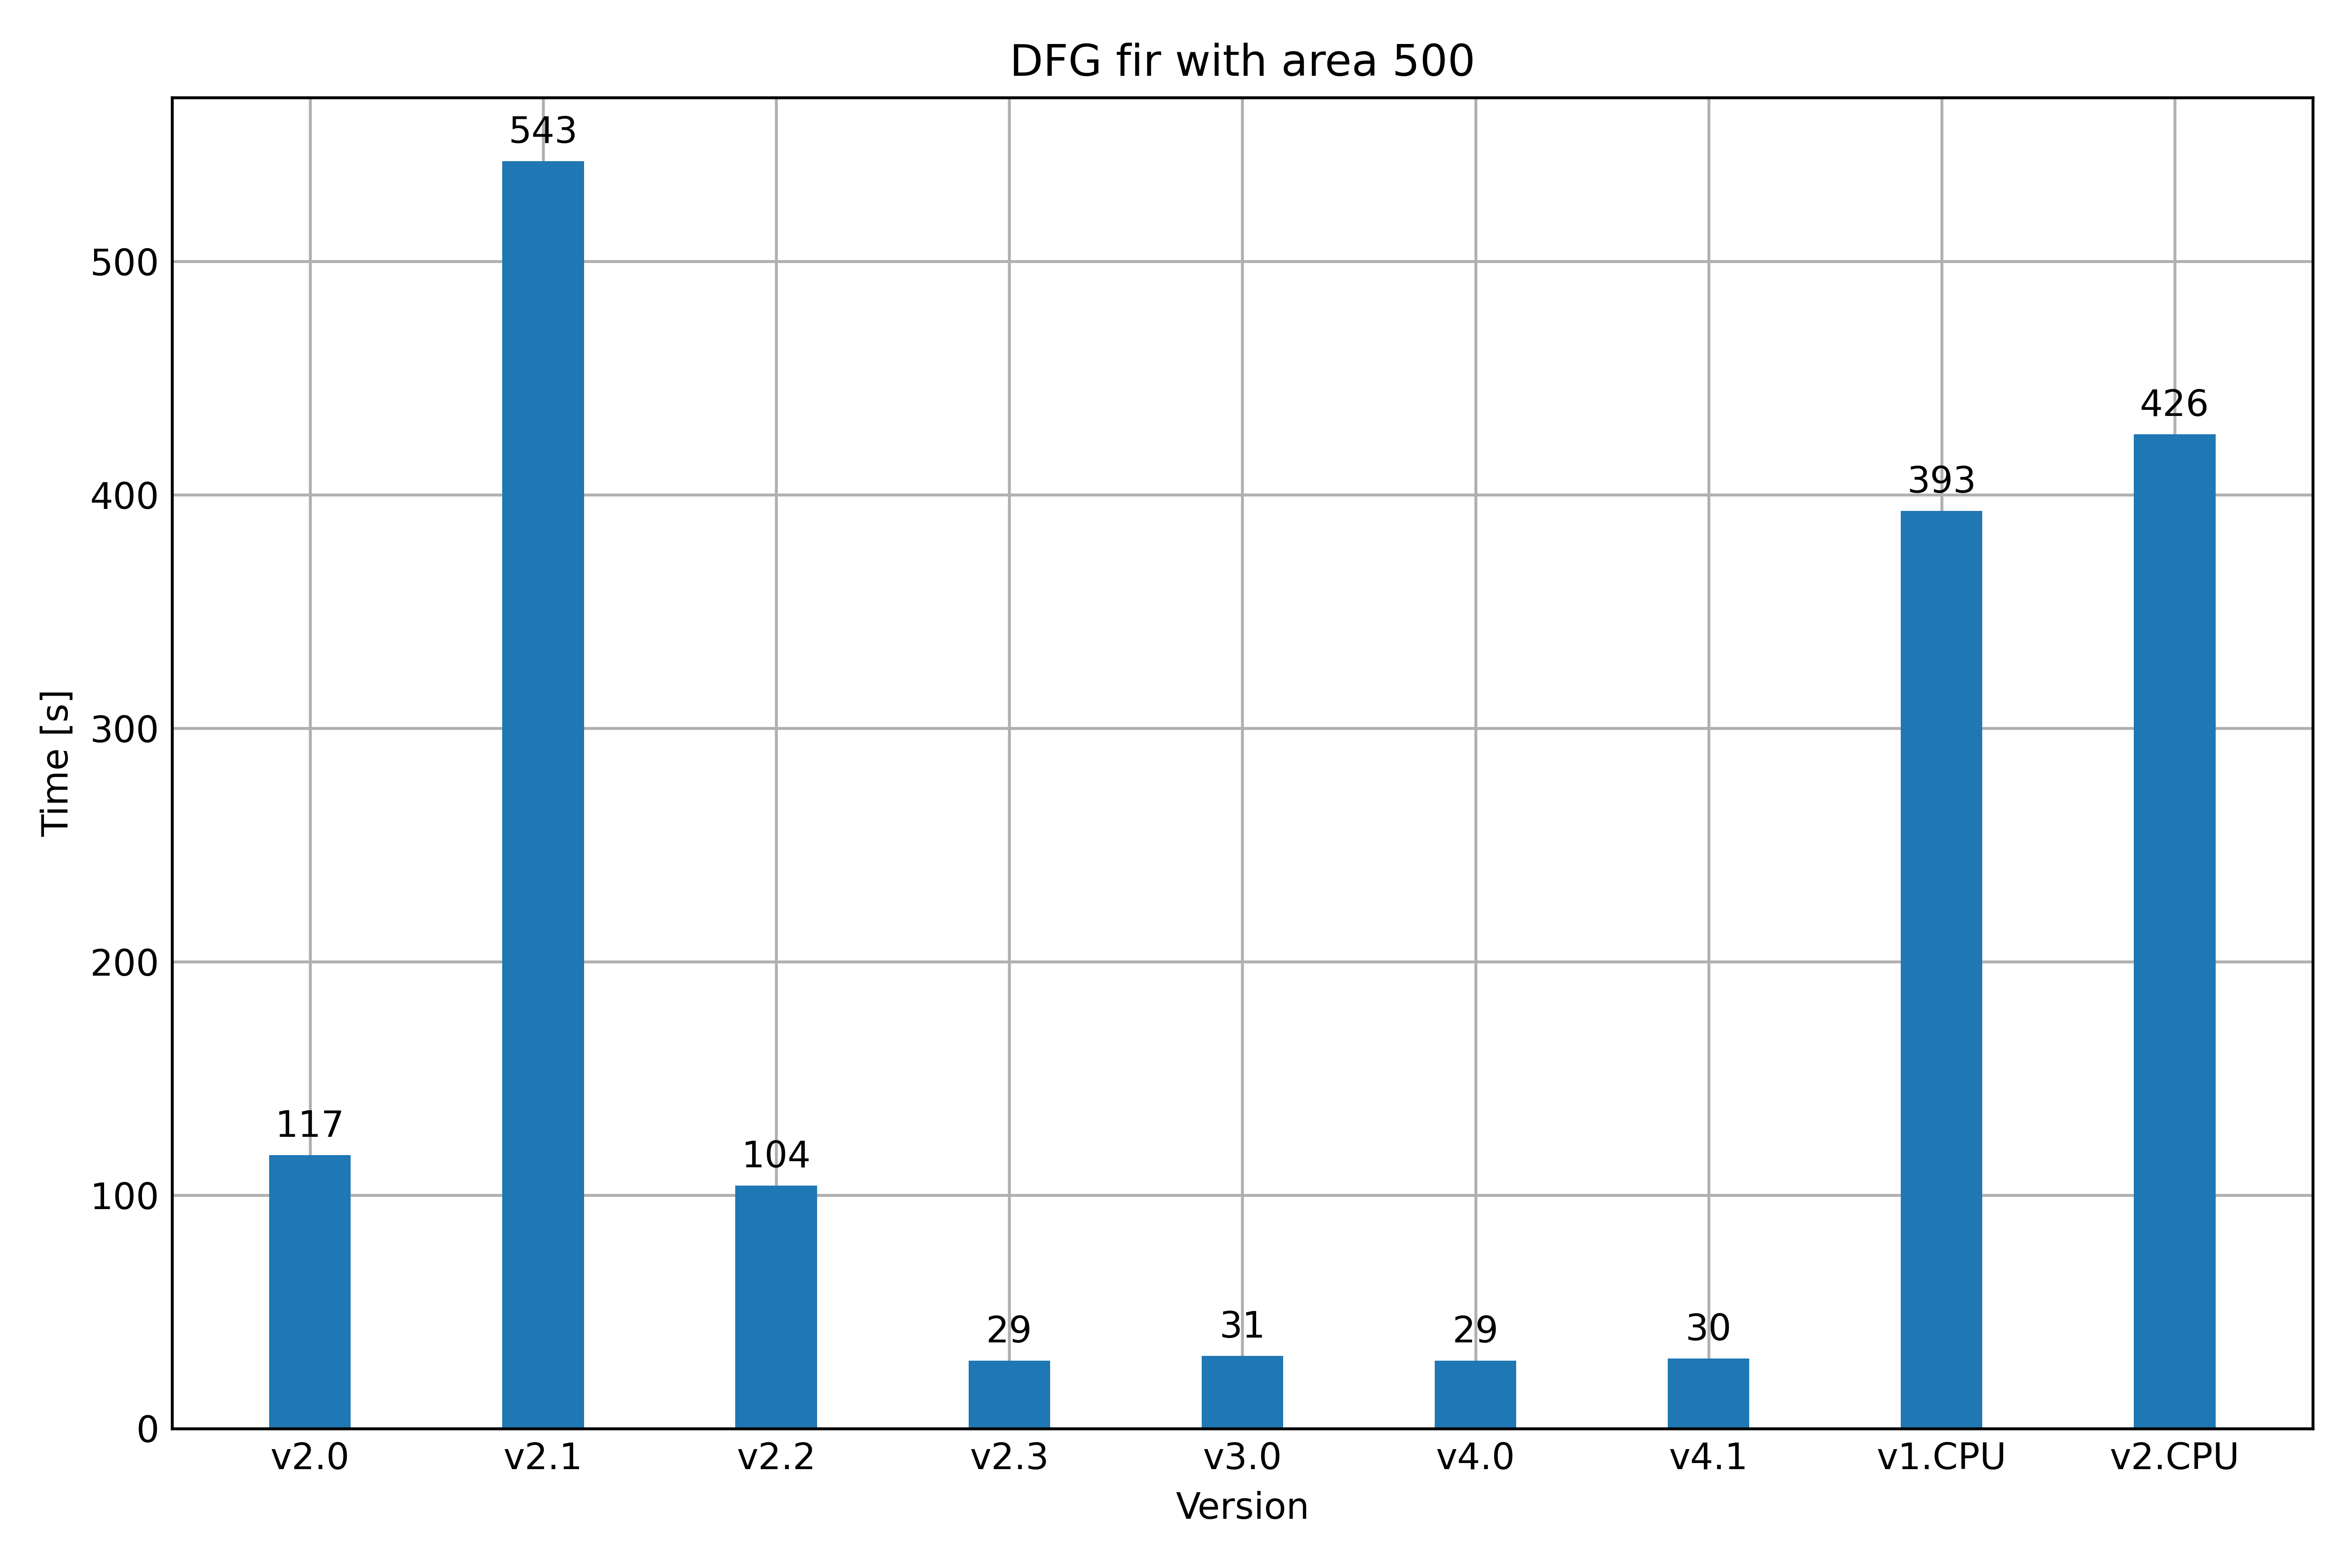
\includegraphics[width=.95\linewidth]{chapters/figures/fir_500.png}  
        \caption{fir bar graph with area 500}
        \label{fig:fir_500}
    \end{subfigure}
    \begin{subfigure}{.45\textwidth}
        \centering
        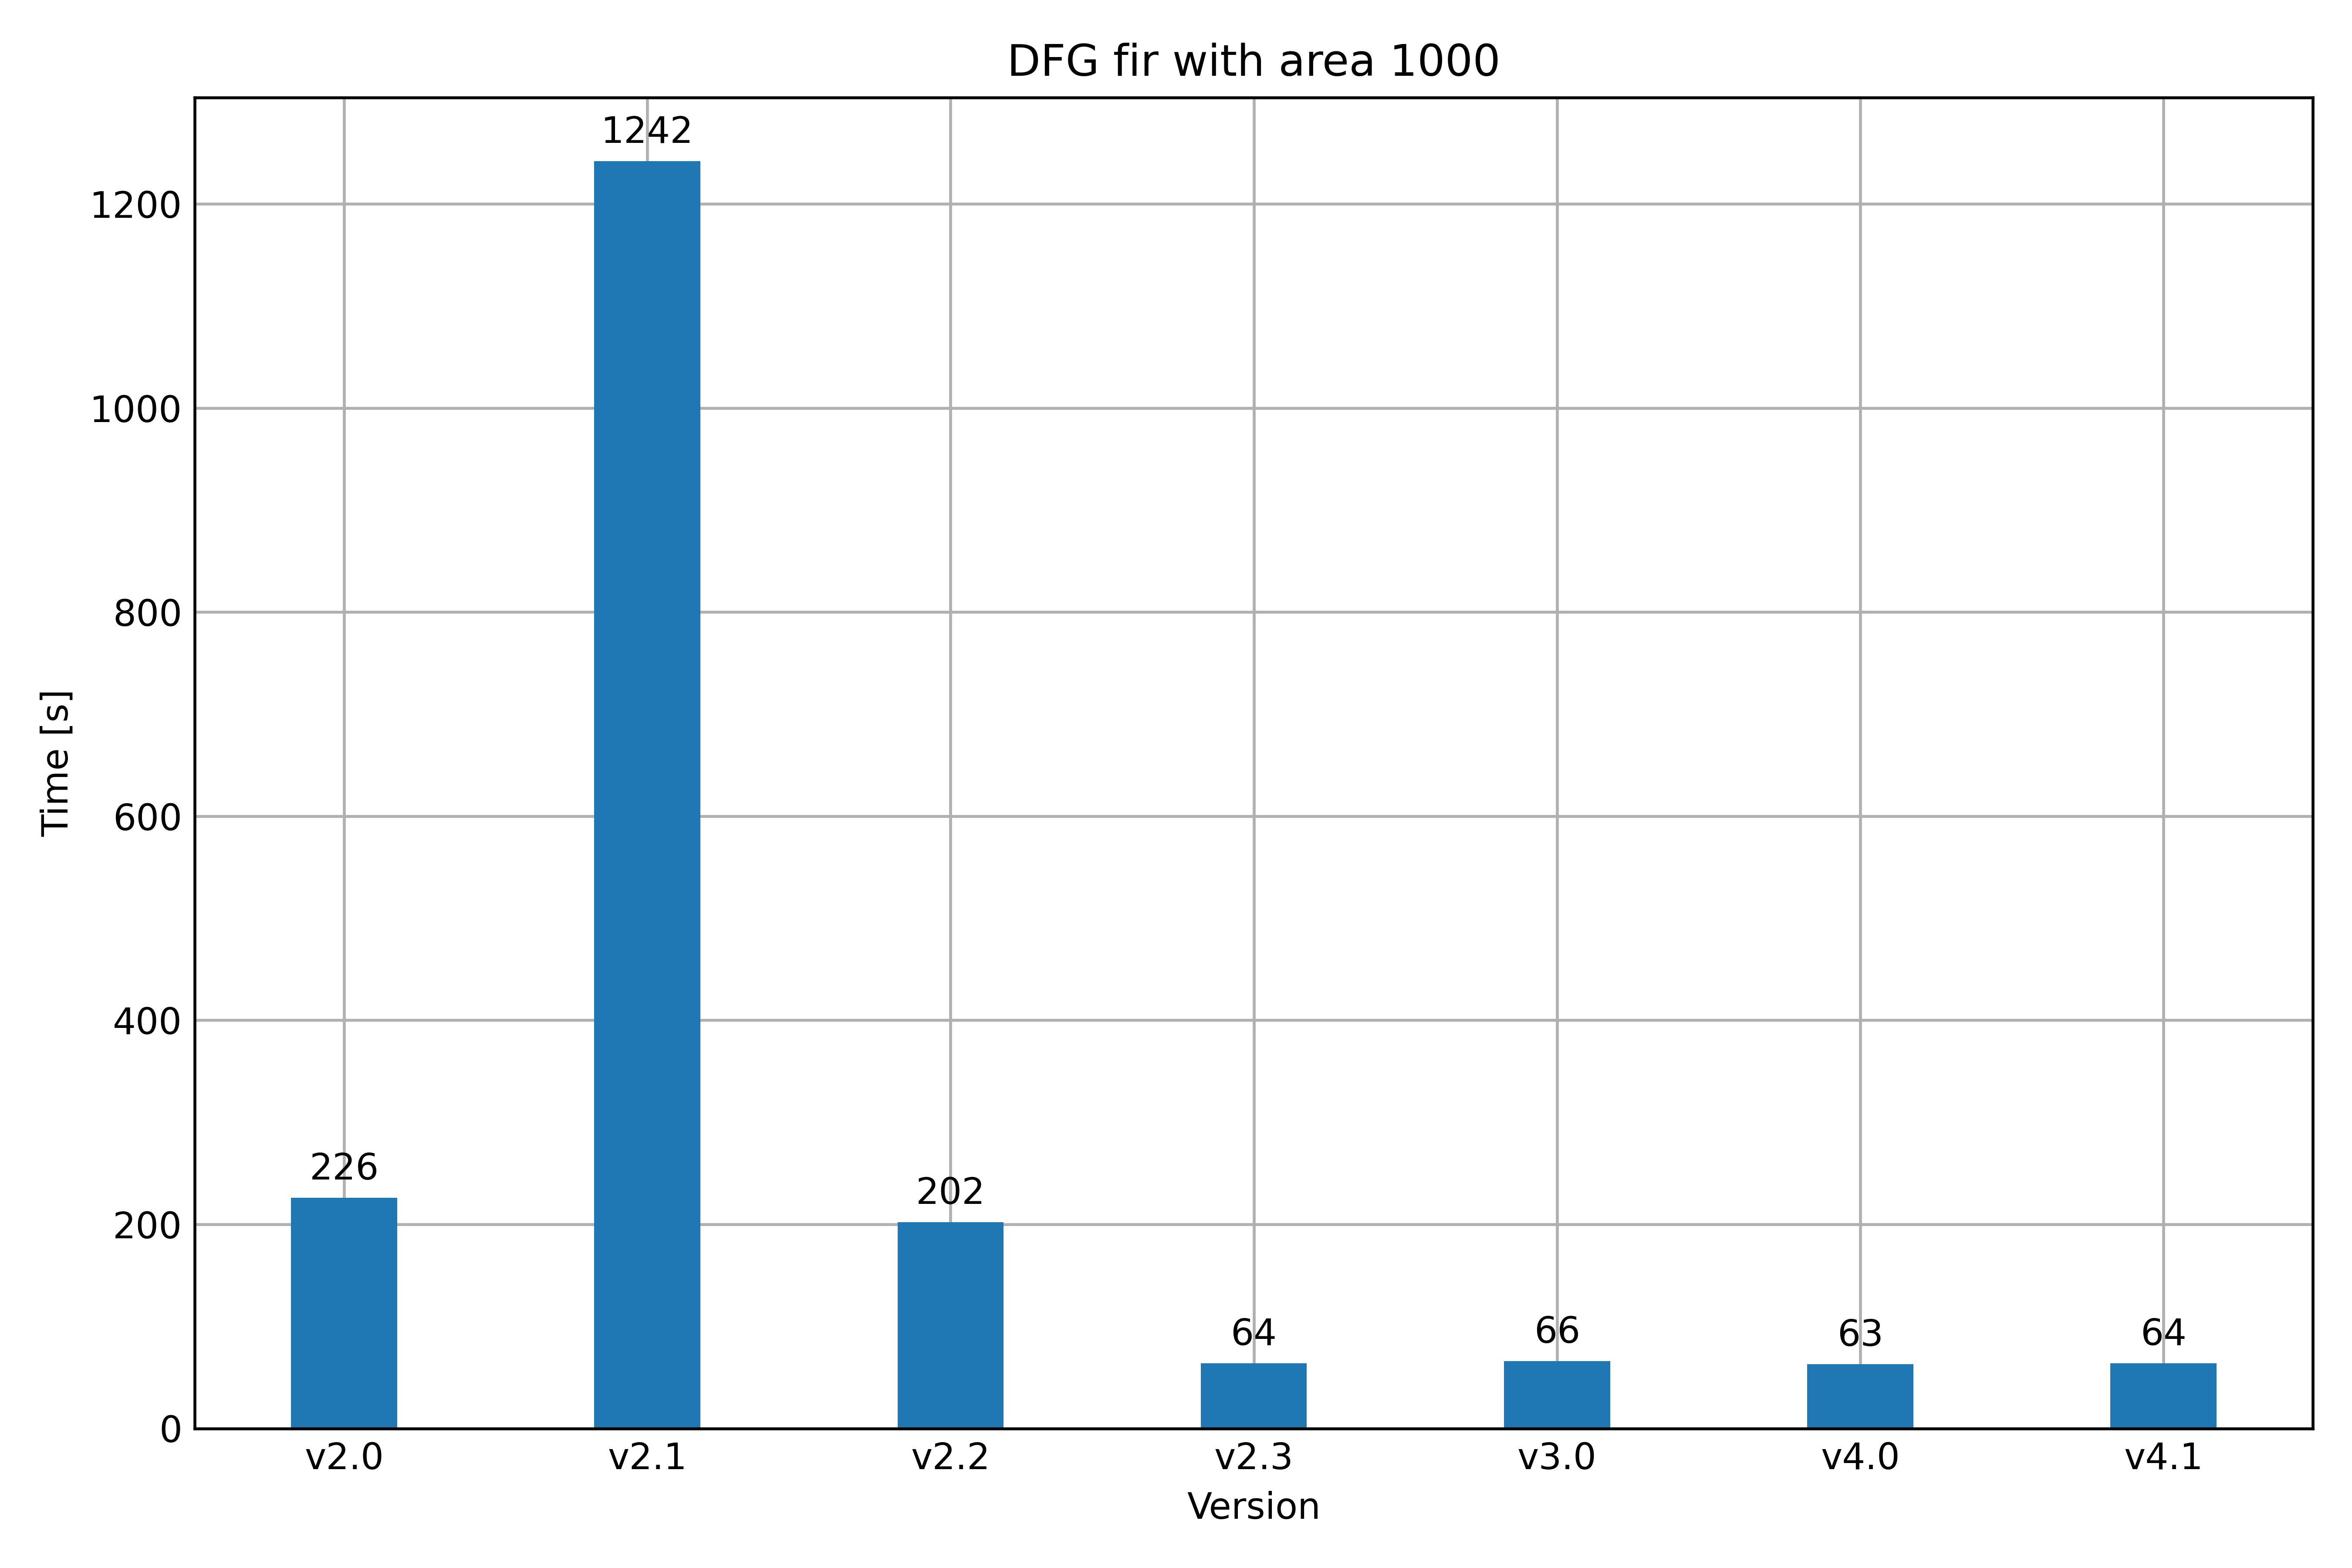
\includegraphics[width=.95\linewidth]{chapters/figures/fir_1000.png}  
        \caption{fir bar graph with area 1000}
        \label{fig:fir_1000}
    \end{subfigure}
\end{figure}

\begin{figure}[h]
    \centering
    \begin{subfigure}{.45\textwidth}
        \centering
        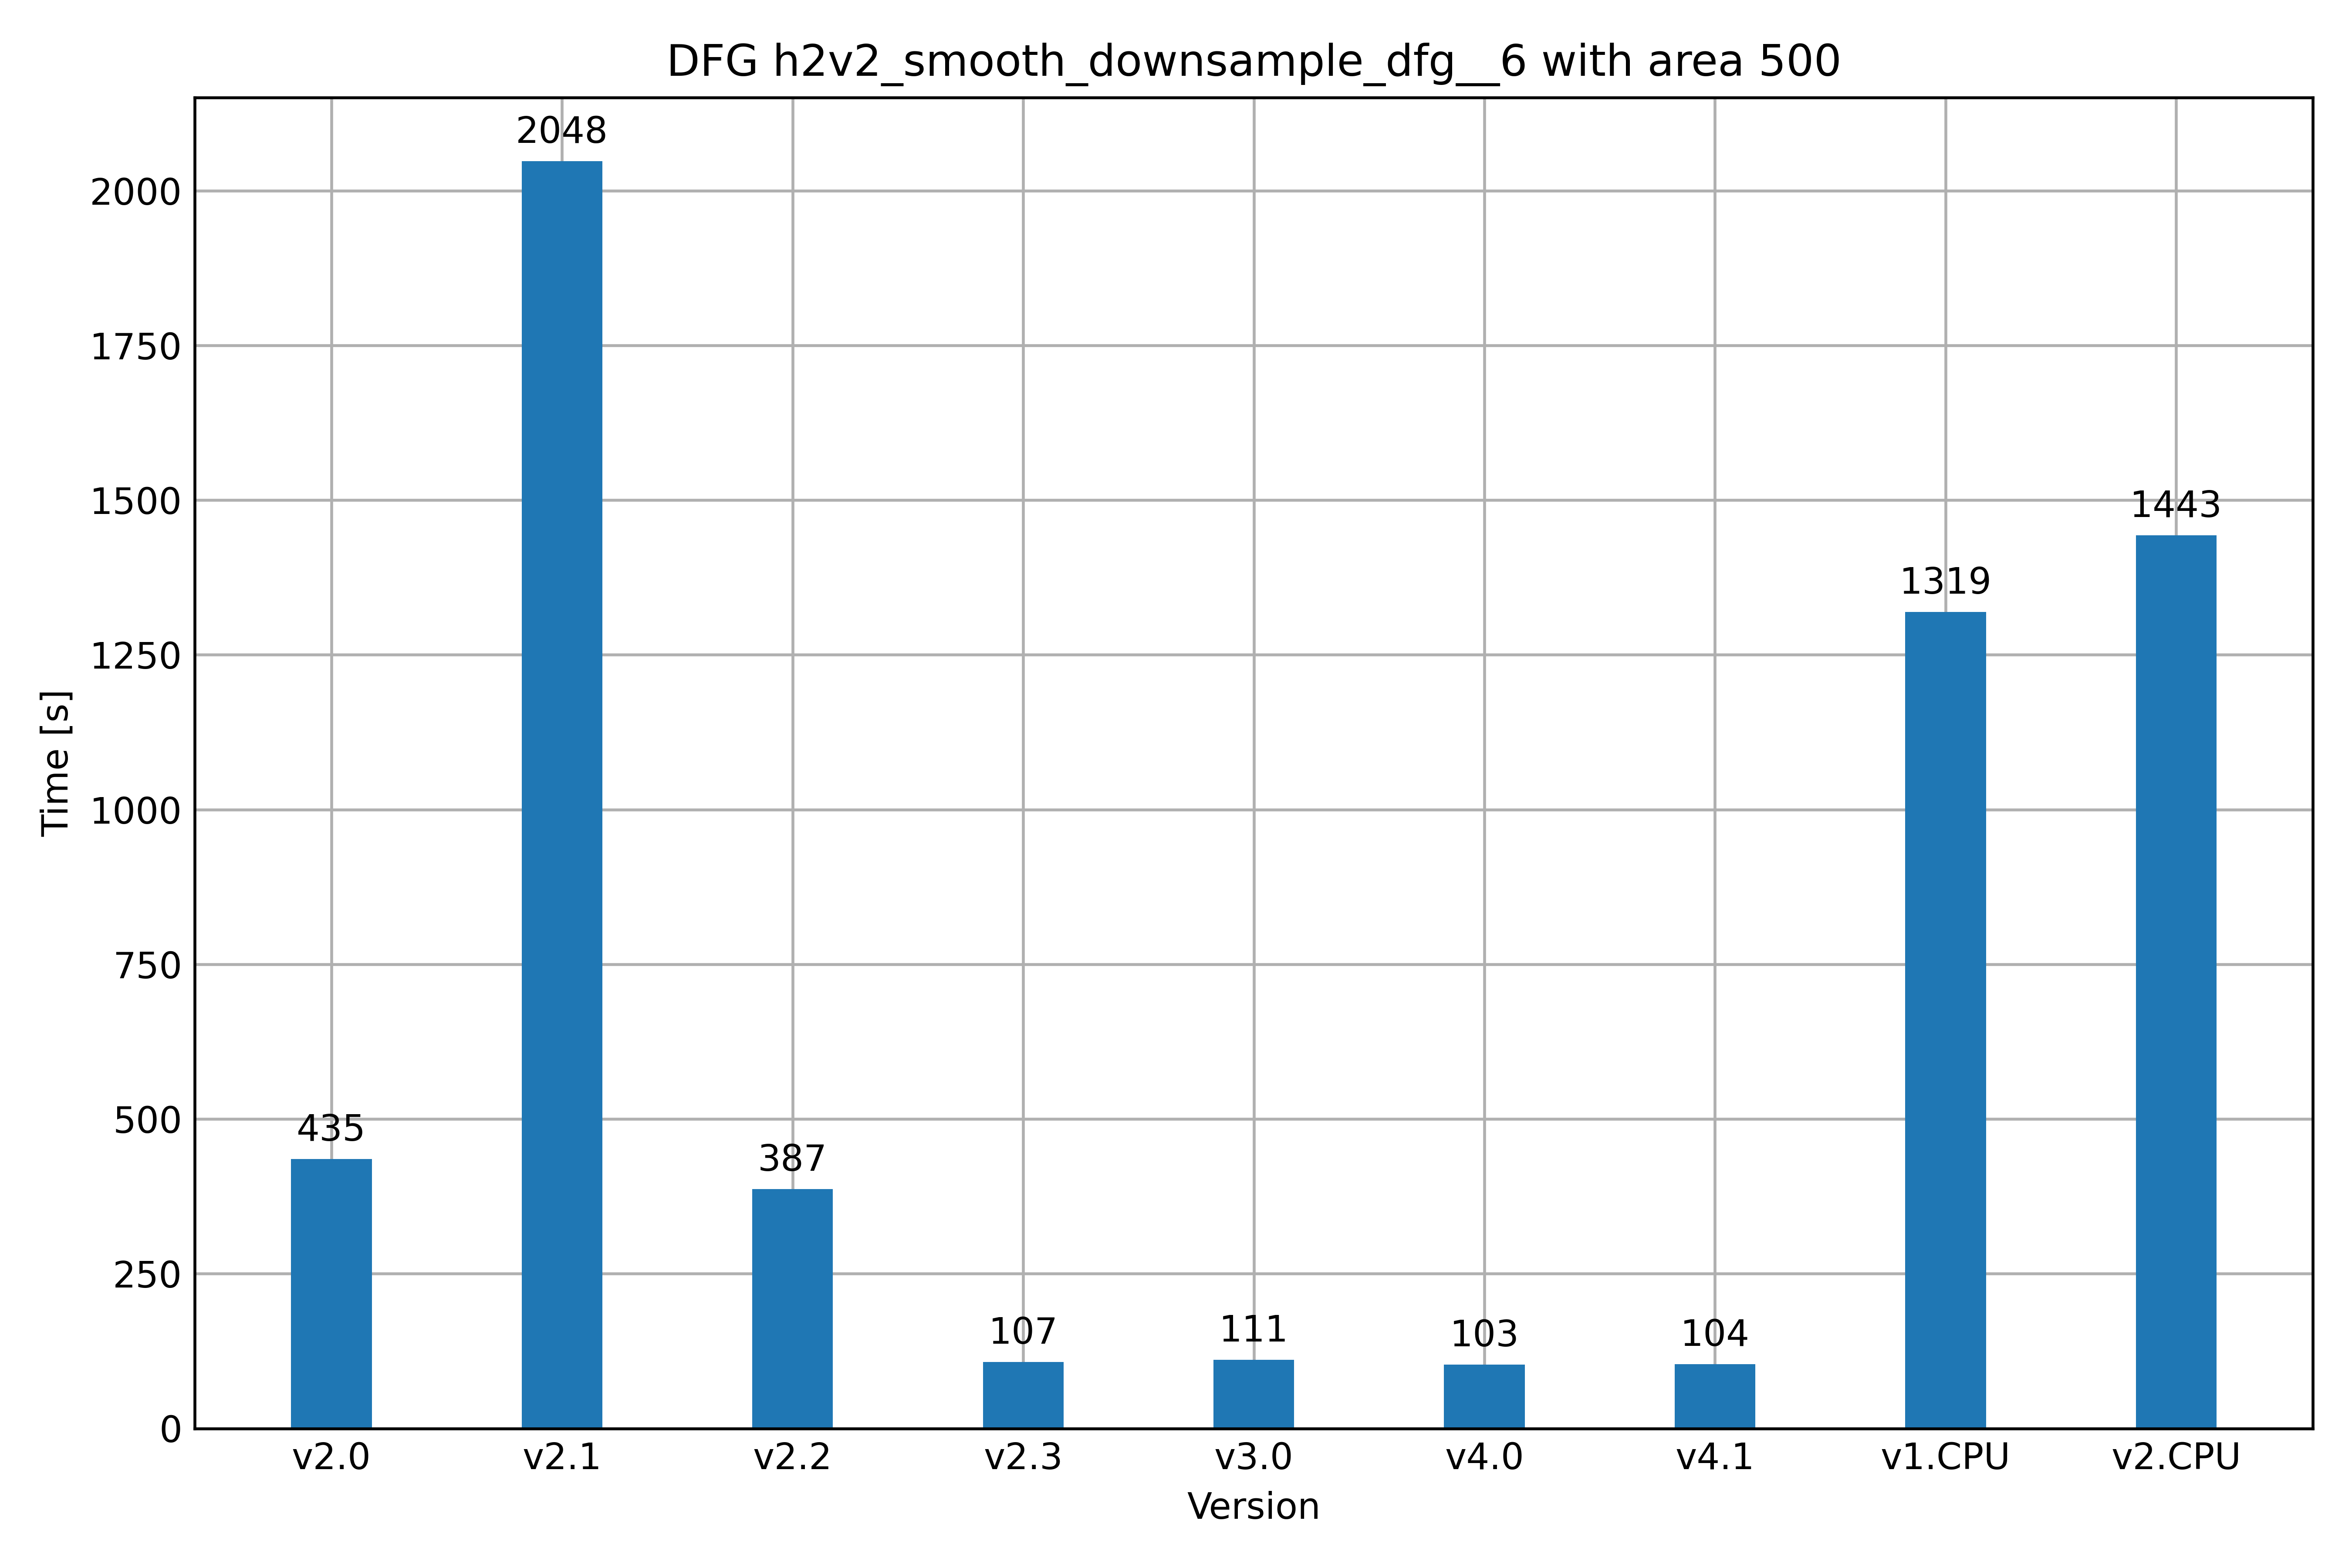
\includegraphics[width=.95\linewidth]{chapters/figures/h2v2_smooth_downsample_dfg__6_500.png}  
        \caption{h2v2 with area 500 bar graph}
        \label{fig:h2v2_500}
    \end{subfigure}
    \begin{subfigure}{.45\textwidth}
        \centering
        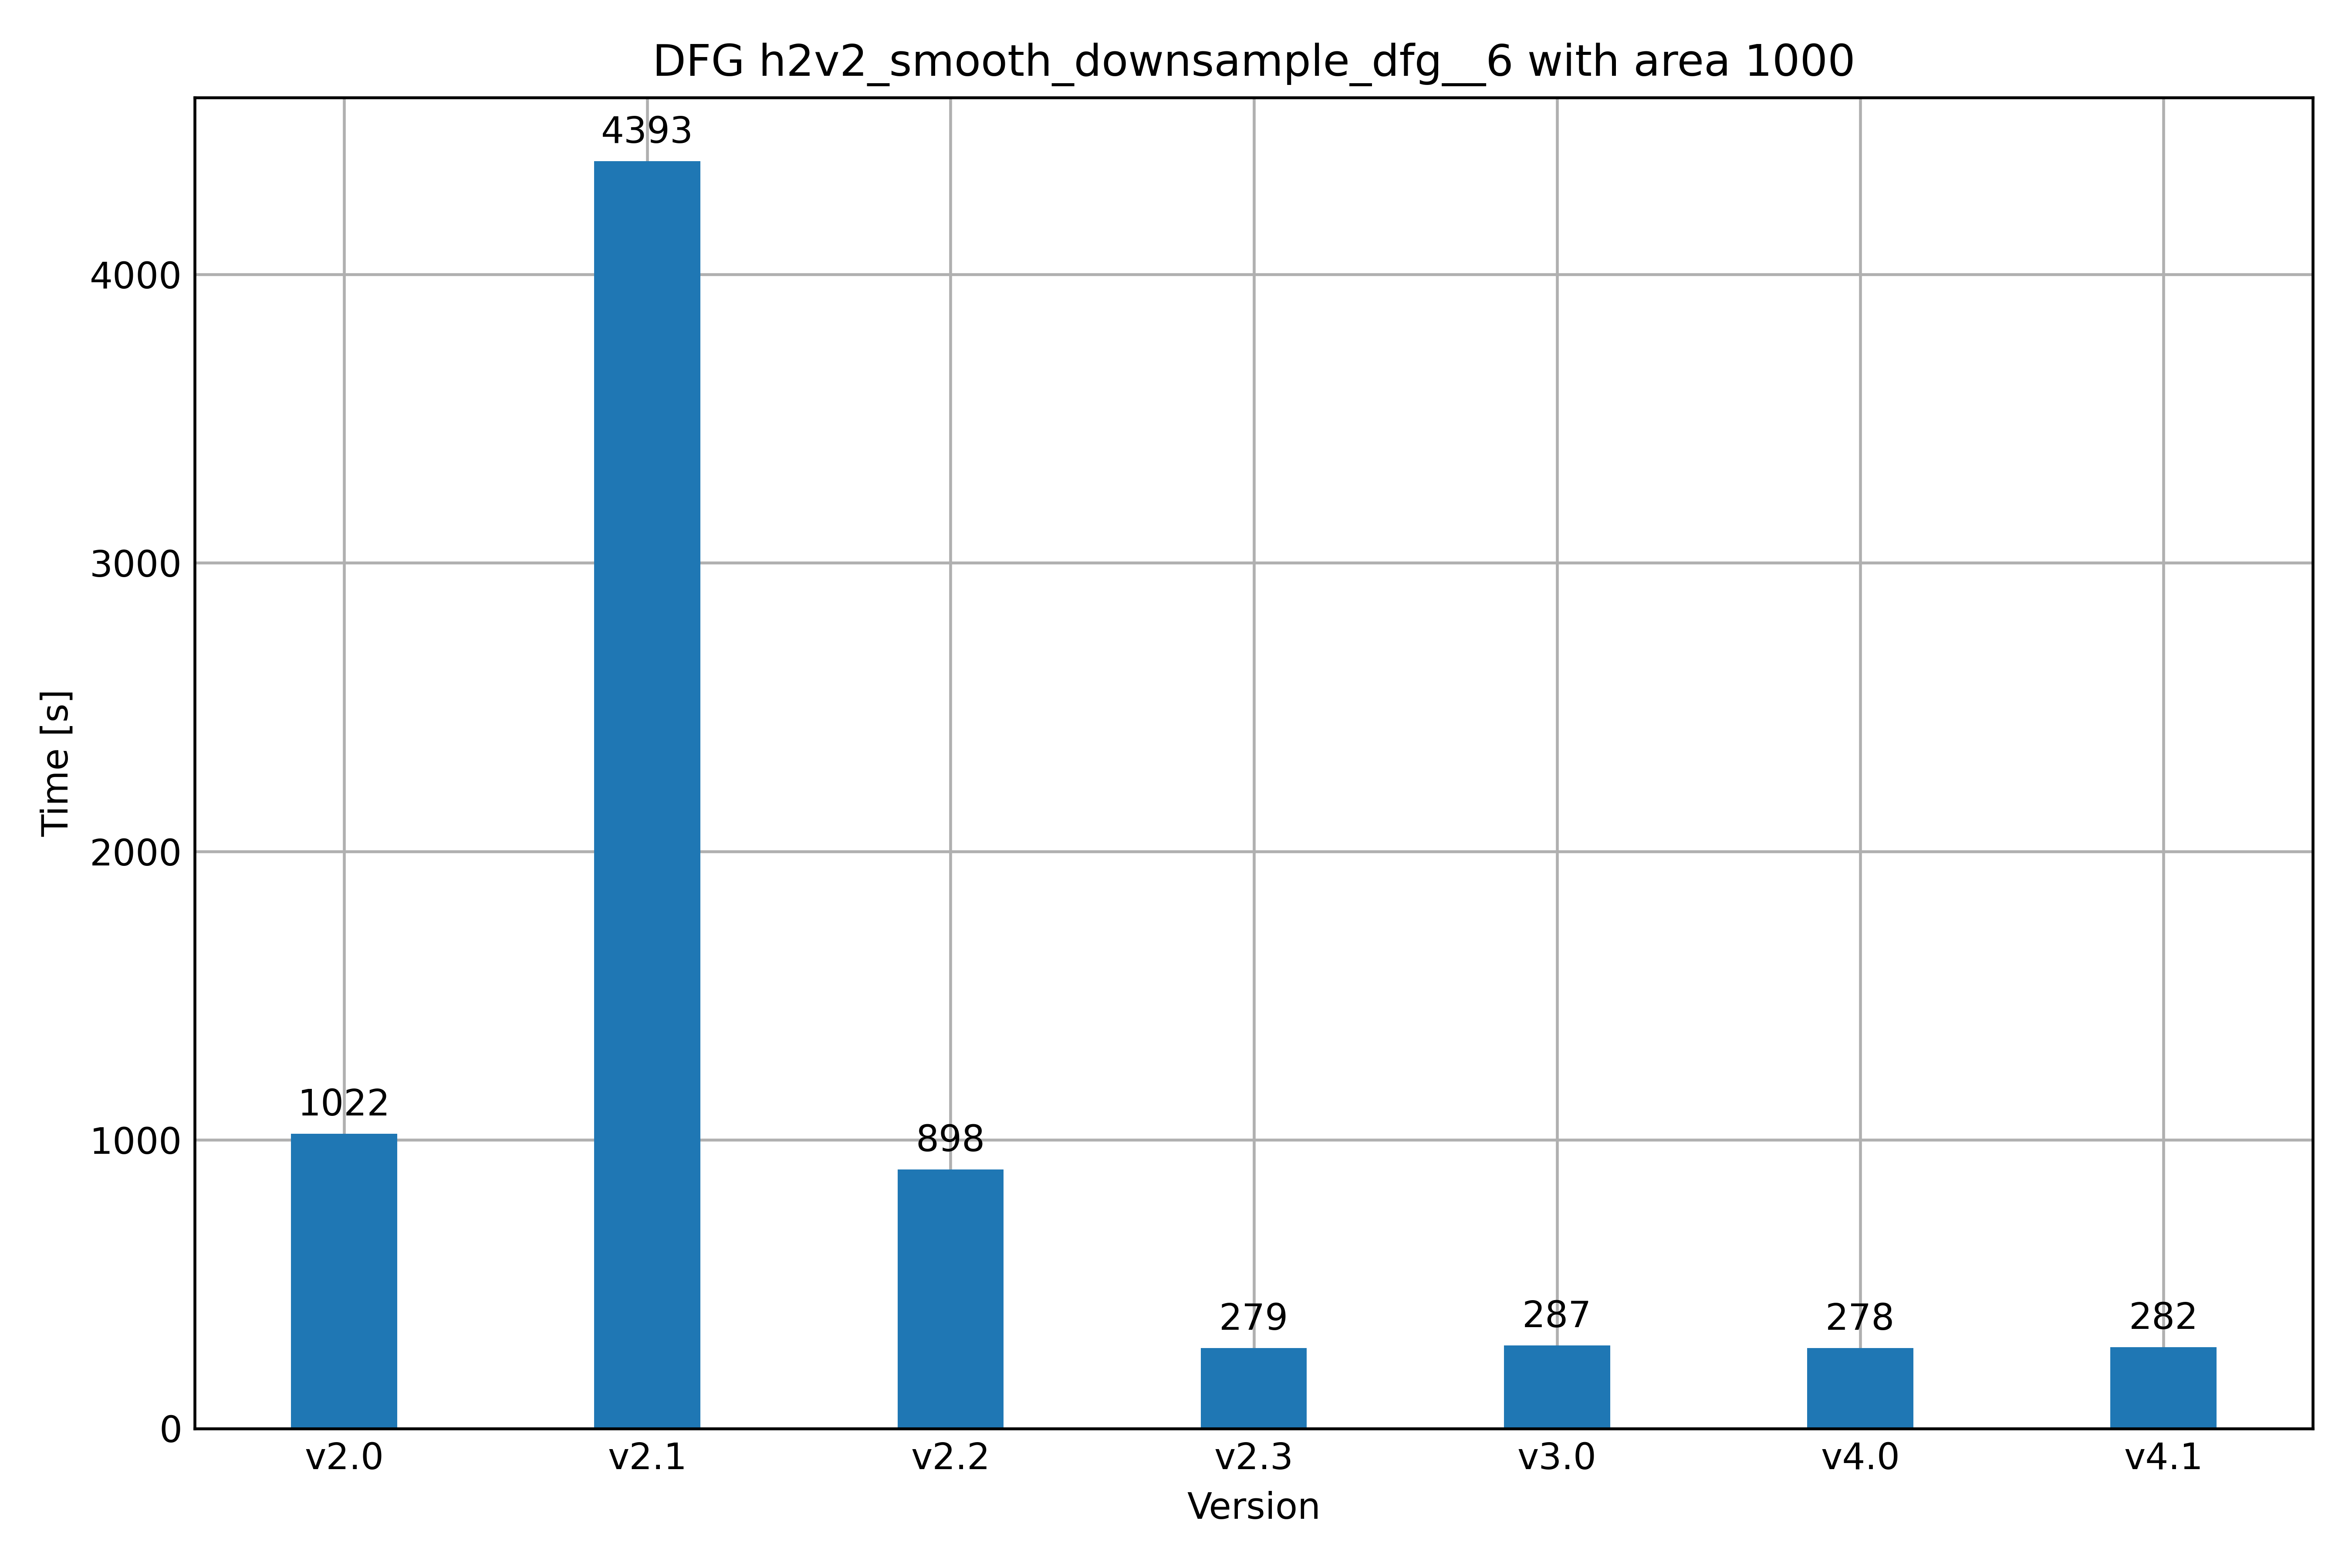
\includegraphics[width=.95\linewidth]{chapters/figures/h2v2_smooth_downsample_dfg__6_1000.png}  
        \caption{h2v2 with area 1000 bar graph}
        \label{fig:h2v2_1000}
    \end{subfigure}
\end{figure}

In the figure \ref{fig:fir_500} it's possible to appreciate the advantage to exploit GPU. Beside the version 2.1 
spent the greatest time, all the others have significant improvement in time, also respect to the first basic version 2.0.

More precise data are avaible in respository folder.

\section{Conclusion}

The code running on GPU respect to the CPU is speed up of 14 times, that is an important quantity.

The final version, that take care of all possible workload problems, is the 4.1 that is a little heavier than 
the 4.0 cause to this little overhead. All the other final version, like 2.3 and 3.0, don't look to have a big 
differences in percentage improvement but, on long execution time, important speed up could be achieved in 4.0.
